\documentclass[12pt,a4paper]{report}

% ================================================================
% ShilpoHubBD Project Report
% Put screenshot files inside docs/images/ and replace the file names
% used by \reportimage. If an image is missing, a placeholder box is
% shown automatically, so the document can still compile.
% ================================================================

\usepackage[utf8]{inputenc}
\usepackage[T1]{fontenc}
\usepackage{lmodern}
\usepackage{geometry}
\usepackage{graphicx}
\usepackage{float}
\usepackage{booktabs}
\usepackage{array}
\usepackage{longtable}
\usepackage{tabularx}
\usepackage{enumitem}
\usepackage{xcolor}
\usepackage{hyperref}
\usepackage{fancyhdr}
\usepackage{listings}
\usepackage{tikz}
\usetikzlibrary{arrows.meta,positioning,shapes.geometric}

\geometry{top=1in,bottom=1in,left=1in,right=1in}
\setlength{\parindent}{0pt}
\setlength{\parskip}{6pt}
\renewcommand{\arraystretch}{1.25}
\setlist[itemize]{leftmargin=1.8em,itemsep=3pt,topsep=4pt}
\setlist[enumerate]{leftmargin=2em,itemsep=3pt,topsep=4pt}

\definecolor{shilpogreen}{HTML}{176B4D}
\definecolor{shilpogold}{HTML}{C58B2B}
\definecolor{softgray}{HTML}{F3F5F4}
\hypersetup{
  colorlinks=true,
  linkcolor=shilpogreen,
  urlcolor=shilpogreen,
  citecolor=shilpogreen,
  pdftitle={ShilpoHubBD Project Report},
  pdfauthor={ShilpoHubBD Project Team}
}

\pagestyle{fancy}
\fancyhf{}
\fancyhead[L]{ShilpoHubBD}
\fancyhead[R]{Project Report}
\fancyfoot[C]{\thepage}
\renewcommand{\headrulewidth}{0.4pt}

\newcommand{\projectname}{\textbf{ShilpoHubBD}}

% Screenshot helper. Example:
% \reportimage{images/home-page.png}{ShilpoHubBD home page}{fig:home}
\newcommand{\reportimage}[3]{%
\begin{figure}[H]
  \centering
  \IfFileExists{#1}{%
    \includegraphics[width=0.92\textwidth,height=0.52\textheight,keepaspectratio]{#1}%
  }{%
    \fcolorbox{shilpogreen}{softgray}{%
      \parbox[c][5.5cm][c]{0.86\textwidth}{%
        \centering\Large\textbf{Image Placeholder}\\[8pt]
        \normalsize Add your screenshot here:\\[4pt]
        \texttt{#1}%
      }%
    }%
  }
  \caption{#2}
  \label{#3}
\end{figure}
}

\lstset{
  basicstyle=\ttfamily\small,
  backgroundcolor=\color{softgray},
  frame=single,
  breaklines=true,
  columns=fullflexible,
  showstringspaces=false
}

\begin{document}

% ----------------------------------------------------------------
% Cover Page
% ----------------------------------------------------------------
\begin{titlepage}
  \centering
  \vspace*{0.5cm}

  % Replace this box with your university logo if needed.
  \IfFileExists{images/university-logo.png}{
    \includegraphics[width=0.18\textwidth]{images/university-logo.png}
  }{
    \fbox{\parbox[c][2.7cm][c]{2.7cm}{\centering University\\Logo}}
  }

  \vspace{0.7cm}
  {\Large \textbf{[University Name]}\par}
  \vspace{0.15cm}
  {\large Department of Computer Science and Engineering\par}

  \vspace{1.1cm}
  {\Huge \color{shilpogreen}\textbf{ShilpoHubBD}\par}
  \vspace{0.25cm}
  {\Large An AI-Powered Digital Ecosystem for Bangladesh's\\Heritage, Crafts, Commerce, Tourism, Learning, and Innovation\par}

  \vspace{1cm}
  \begin{tabular}{|p{0.23\textwidth}|p{0.58\textwidth}|}
    \hline
    \textbf{Course Title} & [Enter Course Title] \\ \hline
    \textbf{Course Code} & [Enter Course Code] \\ \hline
    \textbf{Section} & [Enter Section] \\ \hline
    \textbf{Course Teacher} & [Enter Teacher Name] \\ \hline
  \end{tabular}

  \vspace{0.9cm}
  {\Large \textbf{Team Name: [Enter Team Name]}\par}
  \vspace{0.4cm}

  \begin{tabular}{|p{0.48\textwidth}|p{0.27\textwidth}|}
    \hline
    \textbf{Student Name} & \textbf{Student ID} \\ \hline
    [Student 1] & [ID] \\ \hline
    [Student 2] & [ID] \\ \hline
    [Student 3] & [ID] \\ \hline
    [Student 4] & [ID] \\ \hline
  \end{tabular}

  \vfill
  \textbf{Project Repository}\\
  \url{[Insert GitHub Repository URL]}
\end{titlepage}

\pagenumbering{roman}
\tableofcontents
\clearpage
\listoffigures
\clearpage

% ----------------------------------------------------------------
% Program Outcomes
% ----------------------------------------------------------------
\chapter*{Mapped Program Outcomes}
\addcontentsline{toc}{chapter}{Mapped Program Outcomes}

\begin{longtable}{>{\bfseries}p{0.17\textwidth}p{0.75\textwidth}}
\caption{Program Outcome Mapping for ShilpoHubBD}\\
\toprule
Program Outcome & Project Alignment \\
\midrule
\endfirsthead
\toprule
Program Outcome & Project Alignment \\
\midrule
\endhead
PO2: Problem Analysis &
The project studies connected problems in Bangladesh's heritage and creative economy: limited digital reach for artisans, weak product traceability, fragmented tourism information, limited learning access, difficult business partnerships, and the risk of losing cultural knowledge. These problems are converted into clear software modules and role-based workflows. \\

PO3: Design and Development of Solutions &
The system uses a layered full-stack design with role-based workspaces, REST APIs, relational data, AI-assisted services, logistics coverage, order tracking, heritage research, learning, tourism, and administration. The design supports future growth without placing every responsibility in one component. \\

PO5: Modern Tool Usage &
The project uses React 19, Vite 6, Tailwind CSS, ASP.NET Core 8, Entity Framework Core, PostgreSQL on Supabase, Python, FastAPI, LangChain, Qdrant, Gemini, Leaflet, Nominatim, OSRM, Git, and automated validation scripts. \\

PO8: Ethics &
JWT authentication, BCrypt password hashing, role-based API authorization, audit logs, identity and profile review, product moderation, complaint analysis, source-grounded RAG answers, and rule-based fallbacks support responsible use. AI output is treated as assistance and not as unquestioned truth. \\

PO9: Individual and Teamwork &
The repository is divided into frontend, backend, data, infrastructure, RAG, documentation, tests, and tooling. This separation lets team members work on independent areas while following shared API contracts and domain rules. \\

PO10: Communication &
The project uses DTOs, validators, Swagger/OpenAPI, readable route names, structured dashboards, technical documentation, tests, and this report to explain the system to both technical and non-technical readers. \\

PO12: Life-long Learning &
Development required learning modern AI retrieval, vector databases, prompt design, geographic APIs, secure web APIs, cloud PostgreSQL, logistics state machines, and multi-role business workflows. \\
\bottomrule
\end{longtable}

% ----------------------------------------------------------------
% Abstract
% ----------------------------------------------------------------
\chapter*{Abstract}
\addcontentsline{toc}{chapter}{Abstract}

ShilpoHubBD is a large web platform designed to support Bangladesh's artisans, heritage, tourism, learning, research, business partnerships, public organizations, and digital marketplace activities in one connected system. It provides separate workspaces for customers, producers, business partners, tourists, Heritage Academy members, Heritage Innovation Hub members, Government/NGO users, logistics operations, and Super Administrators.

The system combines an e-commerce marketplace with artisan profiles, product stories, custom orders, auctions, tourism planning, heritage discovery, courses, mentorship, research tools, government monitoring, verified organization support, and location-based delivery. Artificial intelligence is used in product intelligence, semantic product search, review moderation, repeated complaint detection, tourism planning, translation, heritage question answering, product image analysis, producer impact analysis, and other decision-support features. The platform uses React for the frontend, ASP.NET Core for the backend, Entity Framework Core with Supabase PostgreSQL for data, and a Python FastAPI service with LangChain and Qdrant for retrieval-augmented generation. The goal is to preserve cultural knowledge while also creating practical economic opportunities for the people and organizations connected to it.

\clearpage
\pagenumbering{arabic}

% ----------------------------------------------------------------
% Main Report
% ----------------------------------------------------------------
\chapter{Introduction}

Bangladesh has a rich tradition of handloom, pottery, woodwork, metalwork, natural fibre crafts, folk art, regional food, festivals, historic places, and community knowledge. Many artisans and heritage communities still depend on local markets, manual records, and informal communication. Customers may not know the maker or cultural meaning of a product. Tourists often search across many sources to plan a journey. Researchers, training organizations, businesses, and government bodies also need reliable and connected data.

\projectname{} was developed as a single digital ecosystem for these needs. It joins public heritage discovery, online commerce, tourism, education, research, logistics, governance, and AI-assisted tools. The platform follows a modular architecture so that each business area has its own domain entities, services, repositories, API controllers, DTOs, validation rules, and frontend pages while still sharing identity, authorization, messaging, notifications, and common data.

\chapter{Motivation}

The main motivation is to make Bangladesh's cultural and creative economy more visible, trusted, and connected. The project addresses the following practical needs:

\begin{itemize}
  \item Give producers a digital place to present products, stories, skills, and production capacity.
  \item Help customers buy authentic products and understand their cultural background.
  \item Support business partnerships, procurement, contracts, quotations, sponsorship, investment, and supplier discovery.
  \item Help tourists discover places, crafts, food, routes, services, and festivals using maps and an AI trip planner.
  \item Provide courses, mentorship, apprenticeships, assessments, certificates, and portfolios through the Heritage Academy.
  \item Give researchers and the Heritage Innovation Hub structured data, projects, surveys, publications, knowledge graphs, and experimental tools.
  \item Give Government/NGO users dashboards, monitoring, funding, reporting, policy tools, and verified artisan-support workflows.
  \item Provide administrators with central control over users, content, verification, security, marketplace quality, official logistics partners, and audits.
  \item Use AI carefully to improve discovery and decision support while keeping important business rules deterministic and auditable.
\end{itemize}

\chapter{Objectives of the System}

The objectives of ShilpoHubBD are:

\begin{enumerate}
  \item Build a complete role-based web platform for Bangladesh's heritage and creative economy.
  \item Preserve and present cultural information about crafts, districts, villages, producers, stories, festivals, museum items, and UNESCO-related records.
  \item Provide marketplace functions such as products, categories, cart, wishlist, checkout, order history, returns, refunds, reviews, auctions, and custom orders.
  \item Connect producers with customers, business partners, academy members, researchers, logistics companies, and public organizations.
  \item Provide database-driven delivery availability based on Division, District, and Upazila/Area.
  \item Support real delivery tracking, delivery history, partner performance, and logistics revenue sharing.
  \item Provide tourism discovery, booking, route planning, map services, and saved trip plans.
  \item Provide learning, mentorship, apprenticeship, live classes, assessment, certification, and portfolio tools.
  \item Provide research, innovation, field survey, heritage database, knowledge graph, and publication workflows.
  \item Use AI and retrieval systems for grounded assistance, search, classification, forecasting, matching, analysis, and content support.
  \item Protect data through authentication, authorization, validation, moderation, audit logging, and safe configuration practices.
\end{enumerate}

\chapter{System Overview}

ShilpoHubBD is a browser-based single-page application. The React frontend sends HTTP requests to ASP.NET Core REST APIs. The backend applies authorization and business rules, then reads or writes data through Entity Framework Core. The primary relational database is PostgreSQL hosted through Supabase. A separate Python FastAPI service provides heritage and product retrieval using LangChain and Qdrant. Gemini is used only by configured providers; many sensitive decisions still use deterministic rules or explicit fallbacks.

\section{User Roles}

\begin{longtable}{p{0.24\textwidth}p{0.68\textwidth}}
\toprule
\textbf{Role} & \textbf{Main Responsibility} \\
\midrule
Customer & Discover and buy products, follow producers, manage orders, returns, reviews, community activity, and AI shopping tools. \\
Producer & Manage products, stock, orders, custom work, auctions, stories, sustainability, partnerships, academy activity, and support cases. \\
Business Partner & Manage procurement, contracts, quotations, supplier discovery, investments, sponsorship, partnerships, analytics, and product intelligence. \\
Tourist & Explore heritage and tourism information, use maps and routes, book services, save plans, use the travel passport, and use the AI planner. \\
Heritage Academy Member & Join courses, learning plans, mentorship, live classes, quizzes, exams, assignments, certificates, and portfolios. \\
Heritage Innovation Hub & Manage research projects, datasets, publications, experiments, prototypes, preservation work, surveys, and the knowledge graph. \\
Government/NGO & Use national dashboards, monitoring, reports, funding, policy simulation, compliance, complaints, heritage data, and artisan support. This account is created by a Super Administrator and is not publicly self-registered. \\
Logistics Operations & Manage warehouses, shipments, stock, pickup requests, returns, routes, and logistics decision-support tools. Official company and coverage configuration is controlled by an administrator. \\
Super Administrator & Manage users, profiles, content, marketplace moderation, security, official logistics partners, governance oversight, and system-wide reports. \\
\bottomrule
\end{longtable}

\section{High-Level Architecture}

\begin{figure}[H]
\centering
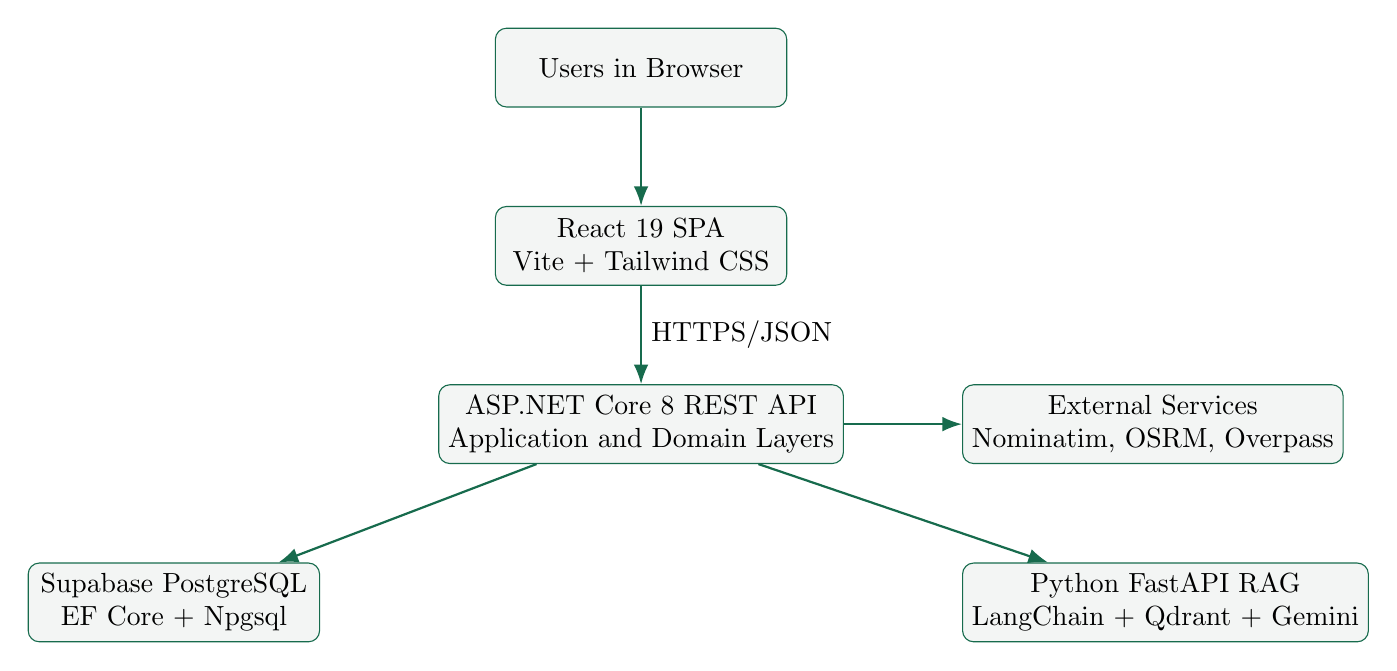
\begin{tikzpicture}[
  node distance=1.25cm and 1.5cm,
  box/.style={draw=shilpogreen,rounded corners,fill=softgray,minimum width=3.7cm,minimum height=1.0cm,align=center},
  arrow/.style={-{Latex[length=2.5mm]},thick,draw=shilpogreen}
]
\node[box] (user) {Users in Browser};
\node[box,below=of user] (front) {React 19 SPA\\Vite + Tailwind CSS};
\node[box,below=of front] (api) {ASP.NET Core 8 REST API\\Application and Domain Layers};
\node[box,below left=of api] (db) {Supabase PostgreSQL\\EF Core + Npgsql};
\node[box,below right=of api] (rag) {Python FastAPI RAG\\LangChain + Qdrant + Gemini};
\node[box,right=of api] (external) {External Services\\Nominatim, OSRM, Overpass};
\draw[arrow] (user) -- (front);
\draw[arrow] (front) -- node[right]{HTTPS/JSON} (api);
\draw[arrow] (api) -- (db);
\draw[arrow] (api) -- (rag);
\draw[arrow] (api) -- (external);
\end{tikzpicture}
\caption{ShilpoHubBD system architecture}
\label{fig:architecture}
\end{figure}

\chapter{Feature Description}

\section{Public Home and Heritage Discovery}

The public area introduces ShilpoHubBD and gives access to districts, villages, crafts, producers, UNESCO information, museum content, festivals, cultural events, craft stories, and public marketplace information. CMS-managed home sections, blogs, news, events, and announcements allow administrators to keep the site content current.

\reportimage{images/home-page.png}{ShilpoHubBD home page}{fig:home}
\reportimage{images/heritage-explore.png}{Public heritage discovery}{fig:heritage-explore}

\section{Authentication and Role-Based Access}

The platform uses email and password login with JWT access tokens. Passwords are hashed with BCrypt. Backend controllers use role authorization, while frontend routes use role guards. Customers, producers, business partners, tourists, Academy members, and Innovation Hub members can use public registration. Government/NGO accounts are created by a Super Administrator. Public registration for logistics companies is disabled in the official logistics model.

\reportimage{images/login.png}{Login interface}{fig:login}
\reportimage{images/register.png}{Role-based registration interface}{fig:register}

\section{Customer Marketplace}

Customers can browse products and categories, see product details and cultural stories, use a wishlist and cart, check out, view order history, track delivery, submit returns, view refunds, write reviews, follow producers, join discussions, ask questions, and manage a personal heritage collection. The checkout reads real delivery options from configured logistics coverage and validates the selected partner again in the backend.

\reportimage{images/customer-marketplace.png}{Customer marketplace}{fig:customer-marketplace}
\reportimage{images/customer-checkout.png}{Checkout with location-based delivery options}{fig:checkout}
\reportimage{images/customer-order-tracking.png}{Order and delivery tracking timeline}{fig:tracking}

\section{Customer AI Shopping Tools}

The customer workspace includes similar-product discovery, gift recommendation, fashion matching, interior preview, and AI-assisted product search. Product search uses real marketplace data and can use vector candidates from Qdrant. Fashion matching uses structured attributes and real catalog candidates. Interior preview calls a Gemini image-capable provider when the required model is configured. The system returns a controlled error or fallback when a required AI service is not available; it does not present invented products as database records.

\reportimage{images/ai-product-search.png}{AI-assisted product search}{fig:ai-search}
\reportimage{images/ai-fashion-matching.png}{AI fashion matching}{fig:fashion}
\reportimage{images/ai-interior-preview.png}{AI interior preview}{fig:interior}

\section{Producer Workspace}

Producers manage their profile, products, variants, attributes, images, videos, inventory, orders, returns, questions, custom orders, auctions, and live shopping. They can also use contracts, quotations, procurement, design collaboration, product development, CSR sponsorship, investment opportunities, sustainability records, producer intelligence, partnership agreements, settlements, and artisan support cases. Product approval and moderation protect the public catalog.

\reportimage{images/producer-dashboard.png}{Producer dashboard}{fig:producer-dashboard}
\reportimage{images/producer-products.png}{Producer product management}{fig:producer-products}
\reportimage{images/producer-partnerships.png}{Producer partnership workflow}{fig:producer-partnerships}

\section{Business Partner Workspace}

Business partners can create a business profile, find suppliers, compare producers, request quotations, manage procurement and inspections, create contracts, join manufacturing and design partnerships, sponsor CSR work, publish investment opportunities, use partnership auctions, and review analytics. AI and rule-based decision-support features provide demand, price, production, spending, supplier, and product intelligence insights from available data.

\reportimage{images/business-partner-dashboard.png}{Business partner dashboard}{fig:bp-dashboard}
\reportimage{images/business-partner-analytics.png}{Business analytics and intelligence}{fig:bp-analytics}

\section{Tourism and Tourist Workspace}

Tourists can explore tourism locations, heritage places, villages, routes, festivals, cultural events, local cuisine, services, accommodations, and map data. They can book services, keep a travel passport, save trip plans, and use the AI tourism planner. Nominatim provides geocoding, OSRM provides road routing estimates, Overpass provides external points of interest, and Leaflet displays interactive maps. Route estimates are guidance and not live transport schedules.

\reportimage{images/tourism-home.png}{Tourism discovery page}{fig:tourism-home}
\reportimage{images/tourism-map.png}{Interactive heritage and tourism map}{fig:tourism-map}
\reportimage{images/ai-tourism-planner.png}{AI tourism planner}{fig:tourism-ai}

\section{Heritage Academy}

The Academy supports member profiles, course catalogs, lessons, modules, materials, enrollment, learning progress, mentors, mentor matching, mentorship requests, live classes, quizzes, exams, assignments, skill assessments, roadmaps, apprenticeships, certificates, and digital portfolios. Course enrollment stores the selected attendance mode, fee, and payment status. At present, a paid course is recorded as \texttt{DueToMentor}; a complete online course-payment gateway is not yet connected.

\reportimage{images/academy-catalog.png}{Heritage Academy course catalog}{fig:academy-catalog}
\reportimage{images/academy-learning.png}{Academy learning dashboard}{fig:academy-learning}

\section{Heritage Innovation and Research}

The Heritage Innovation Hub includes research projects, members, tasks, notes, milestones, papers, publications, surveys, field evidence, heritage datasets, live heritage database views, the knowledge graph, experiments, prototypes, innovation submissions, and preservation strategies. A research assistant abstraction exists, but its current provider is a deterministic dummy provider rather than a production large-language-model service.

\reportimage{images/research-workspace.png}{Research workspace}{fig:research-workspace}
\reportimage{images/knowledge-graph.png}{Heritage knowledge graph}{fig:knowledge-graph}

\section{Government and NGO Workspace}

Government/NGO users have access to a national dashboard, district rankings, trends, monitoring, funding programs, applications, policy simulation, compliance, complaints, forecasts, reports, heritage intelligence, heritage data, knowledge graphs, producer monthly reports, and artisan support. An organization completes a verified profile before managing assigned artisan-support work. This workflow records inspection, support plans, evidence, delivery confirmation, monitoring, final reports, disputes, flags, and administrative review.

\reportimage{images/government-dashboard.png}{Government and NGO dashboard}{fig:gov-dashboard}
\reportimage{images/artisan-support.png}{Verified artisan-support workflow}{fig:artisan-support}

\section{Official Logistics and Delivery}

The Super Administrator creates official logistics companies and configures company information, service areas, methods, estimated delivery time, charges, pickup support, return support, and active status. Coverage follows the Bangladesh location hierarchy and is stored in the database. Checkout shows only active partners that serve the destination. The backend checks coverage again before order creation.

A delivery stores its partner, tracking number, current status, history, expected time, pickup and delivery time, failure or return reasons, charge, ShilpoHub share, and partner share. Invalid status changes are rejected. ShilpoHub's configured logistics revenue share is 30 percent and is stored with the delivery so later configuration changes do not change historical records.

\reportimage{images/admin-logistics-partners.png}{Administrator logistics partner management}{fig:admin-logistics}
\reportimage{images/logistics-coverage.png}{Division, district, and area coverage configuration}{fig:coverage}
\reportimage{images/logistics-performance.png}{Logistics performance and revenue view}{fig:logistics-performance}

\section{Administration, CMS, and Security}

The Super Administrator manages users, activation status, Government/NGO account creation, profile approval, identity verification, products, repeated complaints, reviews, categories, districts, villages, heritage content, CMS content, tourism data, mentor applications, logistics partners, artisan-support oversight, procurement inspections, producer partnership workflows, audit logs, backups, API keys, threats, and blocked IP addresses. The admin interface uses shared resource definitions and contract tests to keep frontend forms aligned with backend DTOs.

\reportimage{images/admin-dashboard.png}{Super Administrator dashboard}{fig:admin-dashboard}
\reportimage{images/admin-user-management.png}{User and profile management}{fig:admin-users}

\section{Messaging and Notifications}

Authenticated users can use direct messaging, conversations, media attachments, and notifications. Domain changes can create notifications for important events such as review, approval, order, support, or workflow changes. Notification data is stored in PostgreSQL and served through authenticated APIs.

\reportimage{images/messages.png}{Direct messaging interface}{fig:messages}
\reportimage{images/notifications.png}{User notifications}{fig:notifications}

\chapter{Technology Stack}

\section{Architecture Overview}

The backend follows a layered architecture:

\begin{itemize}
  \item \textbf{ShilpoHubBD.Domain}: entities, enums, constants, and core domain concepts.
  \item \textbf{ShilpoHubBD.Application}: DTOs, validators, service interfaces, repository interfaces, and business services.
  \item \textbf{ShilpoHubBD.Data}: EF Core DbContext, entity configurations, repositories, migrations, and seed data.
  \item \textbf{ShilpoHubBD.Infrastructure}: JWT, BCrypt, payments, external APIs, Gemini providers, RAG clients, routing, geocoding, and rule-based providers.
  \item \textbf{ShilpoHubBD.Api}: ASP.NET Core startup, middleware, authorization, health checks, Swagger, and REST controllers.
\end{itemize}

At the time of this report, the backend contains 169 controller source files, about 497 domain-entity source files, and 100 EF Core migrations. These numbers show the size of the repository; they should not be treated as a permanent API or table count because the project continues to change.

\section{Frontend Technologies}

\begin{itemize}
  \item \textbf{React 19}: component-based user interface.
  \item \textbf{Vite 6}: development server and production build tool.
  \item \textbf{JavaScript with JSX}: frontend source language.
  \item \textbf{Tailwind CSS 3}: responsive styling and shared design system.
  \item \textbf{React Router 6}: public, protected, and role-based navigation.
  \item \textbf{TanStack React Query 5}: server-state fetching, caching, loading, error, and mutation handling.
  \item \textbf{Axios}: REST API communication and token handling.
  \item \textbf{Zustand}: lightweight client-side state management.
  \item \textbf{Leaflet}: interactive maps for heritage and tourism.
  \item \textbf{PostCSS and Autoprefixer}: CSS processing.
\end{itemize}

\section{Backend Technologies}

\begin{itemize}
  \item \textbf{.NET 8 and ASP.NET Core 8}: REST API and middleware platform.
  \item \textbf{Entity Framework Core 8}: ORM, migrations, relationships, and transactions.
  \item \textbf{Npgsql EF Core Provider}: PostgreSQL connectivity.
  \item \textbf{FluentValidation 12}: request and business-input validation.
  \item \textbf{JWT Bearer Authentication}: stateless API authentication.
  \item \textbf{BCrypt.Net}: password hashing.
  \item \textbf{Swashbuckle}: Swagger/OpenAPI documentation.
  \item \textbf{ASP.NET Health Checks for Npgsql}: database health monitoring.
  \item \textbf{In-memory cache and typed HttpClient}: caching and external service calls.
  \item \textbf{DotNetEnv}: loading environment variables from the repository configuration.
\end{itemize}

\section{Database and Supabase}

The primary database is PostgreSQL. The configured connection string uses a Supabase database host, and the backend connects through Npgsql and Entity Framework Core. Supabase URL, anonymous key, service-role key, and storage-bucket settings are also present in environment configuration. Database schema changes are versioned through EF Core migrations.

The current codebase also contains local web-root upload flows for some media types. Therefore, it is accurate to say that Supabase PostgreSQL is the active relational database and Supabase storage is configured, but not every existing file-upload path is fully moved to Supabase Storage.

Major data groups include:

\begin{itemize}
  \item users, roles, profiles, identity checks, permissions, API keys, and audits;
  \item districts, villages, heritage places, crafts, stories, festivals, museum and UNESCO records;
  \item products, categories, variants, attributes, inventory, cart, wishlist, orders, payments, returns, refunds, auctions, and reviews;
  \item tourism locations, services, bookings, routes, passports, cuisines, plans, and external source records;
  \item courses, lessons, modules, enrollments, mentors, apprenticeships, assessments, certificates, and portfolios;
  \item research, publications, surveys, datasets, knowledge graphs, experiments, and prototypes;
  \item governance, monitoring, funding, reports, complaints, compliance, forecasts, and artisan support;
  \item logistics partners, service coverage, deliveries, status history, tracking, charges, revenue, warehouses, pickups, routes, and returns.
\end{itemize}

\section{AI and Machine Learning Integration}

ShilpoHubBD uses more than one type of intelligent service. The report separates real external AI, retrieval systems, and deterministic decision-support logic.

\subsection{Gemini-Connected Features}

\begin{itemize}
  \item \textbf{Tourism generation and translation}: Gemini creates structured assistance and translated content when configured, with a controlled fallback provider.
  \item \textbf{General translation}: Gemini translation provider for multilingual text.
  \item \textbf{Interior preview}: Gemini image provider combines a room image and a selected product when an image-capable model is configured.
  \item \textbf{Product intelligence}: Gemini returns structured product analysis; a dummy fallback remains available.
  \item \textbf{Review moderation}: Gemini classifies review risk and moderation signals with a rule-based fallback.
  \item \textbf{Repeated complaint analysis}: Gemini compares a new negative review with real prior complaints; deterministic backend rules make the final risk decision.
  \item \textbf{Producer impact analysis}: Gemini creates structured impact analysis with a rule-based fallback.
\end{itemize}

\subsection{Heritage and Travel RAG}

The Python RAG service uses FastAPI, LangChain, Qdrant, Gemini, and hybrid retrieval. Heritage data is loaded from validated JSON files, normalized, cleaned, divided into small aspect-based chunks, embedded, and stored in Qdrant. Retrieval combines dense vectors with local BM25 sparse vectors and Reciprocal Rank Fusion. Gemini first analyzes the question and later produces an answer only from retrieved context. The response includes source records. English, Bangla, and Romanized Bangla questions are supported through query analysis and translation.

The travel planner can also call the RAG service for location and facility context. The .NET backend communicates with this service through typed HTTP clients.

\subsection{Semantic Product and Review Search}

The product indexing pipeline sends approved catalog records to the Python search service. Qdrant stores searchable product information and attributes. The API uses an internal key for index-worker communication. Similar review retrieval uses a related Python provider so complaint classification is based on stored reviews instead of invented text.

\subsection{Rule-Based and Placeholder AI Providers}

The following modules use deterministic scoring, rules, or placeholder providers in the current implementation. They are useful decision-support features but should not be described as trained production machine-learning models:

\begin{itemize}
  \item producer business assistant and demand/material forecast;
  \item business-partner intelligence and price/production insights;
  \item logistics delivery prediction, route optimization, demand forecast, and warehouse allocation;
  \item counterfeit detection;
  \item government forecast, heritage intelligence, and policy simulation;
  \item recommendation provider where the dummy provider is registered;
  \item research AI assistant;
  \item heritage story generation and sentiment analysis;
  \item rule-based heritage assistant fallback.
\end{itemize}

This provider design is intentional: application interfaces allow a real model to replace a dummy or rule-based implementation later without changing the controllers or domain workflows.

\section{Geographic and External Data Services}

\begin{itemize}
  \item \textbf{OpenStreetMap Nominatim}: converts names and addresses to coordinates with rate control.
  \item \textbf{OSRM}: estimates road routes and distance; it is not a live public-transport schedule.
  \item \textbf{Overpass API}: supplies external points of interest for tourism enrichment.
  \item \textbf{Leaflet}: displays maps in the browser.
  \item \textbf{Gemini API}: text, structured analysis, translation, and configured image operations.
  \item \textbf{Qdrant}: vector and hybrid retrieval store for heritage and marketplace search.
\end{itemize}

\section{Authentication and Security Architecture}

\begin{itemize}
  \item JWT bearer tokens protect authenticated APIs.
  \item BCrypt hashes account passwords.
  \item Controller-level role policies protect sensitive actions.
  \item Frontend role guards prevent navigation to unrelated workspaces.
  \item FluentValidation checks request format and required fields.
  \item Important state changes are checked in application services, not only in the user interface.
  \item Audit logs record administrative activities.
  \item Threat monitoring, blocked IP management, API keys, backup controls, and identity verification are available to administrators.
  \item Secrets are read from environment variables and are not meant to be hard-coded in source files.
\end{itemize}

\section{Payment and Financial Handling}

The registered marketplace payment provider is Cash on Delivery. Order, payment, refund, producer settlement, procurement, investment, sponsorship, and logistics financial records are represented in backend modules. Monetary values use decimal types. Logistics revenue is persisted using a 30 percent ShilpoHub share and a 70 percent partner share. Paid Academy enrollment currently records the fee and \texttt{DueToMentor} status; it does not yet complete an online course payment.

\section{Development and Testing Tools}

\begin{itemize}
  \item Git for version control.
  \item Swagger/OpenAPI for API discovery.
  \item .NET build and console regression projects for backend validation.
  \item Vite production build and a custom source validator for frontend validation.
  \item Node-based admin and launch contract tests.
  \item Selenium Python scripts for customer, producer, and tourist browser flows.
  \item Python unit tests and evaluation datasets for RAG, product search, embeddings, synchronization, and retrieval quality.
  \item PowerShell scripts for starting the complete local system and selected data operations.
\end{itemize}

\chapter{System Testing and Validation}

The project uses build checks, contract tests, regression programs, live API smoke tests, and browser-flow scripts. Recent validation produced the following results:

\begin{itemize}
  \item The complete backend solution built with zero warnings and zero errors.
  \item Frontend source validation passed for 622 modules.
  \item The Vite production build completed successfully.
  \item All 29 admin contract checks passed after resolving an old source-control conflict.
  \item All 8 launch-critical contract checks passed.
  \item Fifteen of seventeen existing backend regression projects passed.
  \item The remaining two regression projects require their fake settlement repositories to implement the newer \texttt{GetApprovedTotalsAsync} interface member before those tests can run.
  \item Live login and representative API checks passed for Customer, Producer, Business Partner, Tourist, Heritage Academy Member, Heritage Innovation Hub, Government/NGO, and Super Administrator accounts.
  \item A real Academy enrollment was stored successfully. It also confirmed the current limitation that paid-course enrollment records \texttt{DueToMentor} instead of processing an online course payment.
\end{itemize}

Important validation areas include authentication, role authorization, product approval, order creation, logistics coverage, unsupported partner rejection, delivery status transitions, revenue recording, tourism routes, RAG retrieval, review moderation, notifications, partnerships, and frontend-backend contract alignment.

\chapter{Challenges}

\begin{itemize}
  \item \textbf{Large business scope}: Connecting commerce, heritage, tourism, learning, research, governance, and logistics requires many related entities and APIs.
  \item \textbf{Role separation}: Each role needs useful access without receiving permission to control another role's private workflow.
  \item \textbf{Data quality}: Heritage and tourism data comes from different structures and sources. Normalization and source tracking are necessary.
  \item \textbf{AI reliability}: Gemini can fail, return unexpected JSON, or reach rate limits. Providers need validation, logging, and deterministic fallbacks.
  \item \textbf{Grounding}: AI answers must use real heritage, product, and review data. The RAG and vector-search pipelines reduce unsupported answers.
  \item \textbf{Geographic accuracy}: Place names can have different spelling. Nominatim, normalized districts, and stored location hierarchy help, but external map results still need review.
  \item \textbf{Financial correctness}: Historical charges, shares, and settlements must remain unchanged when later configuration changes.
  \item \textbf{Test maintenance}: Large interfaces change over time, so fake repositories and contract fixtures must be updated with production interfaces.
  \item \textbf{Cloud and local storage}: Database hosting is on Supabase, while some upload paths still use local web storage. A consistent production storage policy is needed.
\end{itemize}

\chapter{Current Limitations and Future Enhancements}

\begin{itemize}
  \item Add a real online payment gateway for paid Academy courses and, if required, marketplace payments beyond Cash on Delivery.
  \item Complete migration of media uploads to managed object storage such as Supabase Storage.
  \item Replace remaining dummy AI providers with measured, production-ready providers only where AI adds clear value.
  \item Add model monitoring, prompt/version tracking, cost limits, response-quality review, and stronger AI safety evaluation.
  \item Expand Bangla and regional-language support for search, learning, tourism, and accessibility.
  \item Add continuous integration that builds every standalone regression project, frontend contract test, RAG test, and Selenium flow.
  \item Add mobile applications or a progressive web application for low-bandwidth and remote users.
  \item Add richer logistics integrations with official partner APIs for live pickup requests and tracking updates.
  \item Add stronger production observability, distributed caching, queue workers, and deployment automation.
  \item Improve accessibility testing, keyboard navigation, screen-reader support, and performance on low-cost devices.
\end{itemize}

\chapter{Conclusion}

ShilpoHubBD demonstrates how software engineering, cloud data, geographic services, and carefully controlled AI can support Bangladesh's heritage and creative economy. The platform is not only an online shop. It connects artisans, customers, tourists, learners, mentors, researchers, business partners, public organizations, logistics companies, and administrators through shared but role-protected workflows.

Its layered ASP.NET Core backend, React frontend, Supabase PostgreSQL database, and Python RAG service provide a strong technical base. Gemini, Qdrant, LangChain, BM25, Nominatim, OSRM, Overpass, and Leaflet add useful intelligent and geographic capabilities. At the same time, the codebase keeps many important decisions inside explicit business rules and clearly uses fallbacks where production AI is not yet available. With continued work on payments, storage, automation, and production deployment, ShilpoHubBD can become a practical platform for cultural preservation, economic participation, education, tourism, and public decision support in Bangladesh.

\appendix
\chapter{Suggested Screenshot List}

Place your screenshots in the \texttt{docs/images/} directory using the file names below. The report automatically shows a placeholder until each file is added.

\begin{enumerate}
  \item \texttt{home-page.png}
  \item \texttt{heritage-explore.png}
  \item \texttt{login.png}
  \item \texttt{register.png}
  \item \texttt{customer-marketplace.png}
  \item \texttt{customer-checkout.png}
  \item \texttt{customer-order-tracking.png}
  \item \texttt{ai-product-search.png}
  \item \texttt{ai-fashion-matching.png}
  \item \texttt{ai-interior-preview.png}
  \item \texttt{producer-dashboard.png}
  \item \texttt{producer-products.png}
  \item \texttt{producer-partnerships.png}
  \item \texttt{business-partner-dashboard.png}
  \item \texttt{business-partner-analytics.png}
  \item \texttt{tourism-home.png}
  \item \texttt{tourism-map.png}
  \item \texttt{ai-tourism-planner.png}
  \item \texttt{academy-catalog.png}
  \item \texttt{academy-learning.png}
  \item \texttt{research-workspace.png}
  \item \texttt{knowledge-graph.png}
  \item \texttt{government-dashboard.png}
  \item \texttt{artisan-support.png}
  \item \texttt{admin-logistics-partners.png}
  \item \texttt{logistics-coverage.png}
  \item \texttt{logistics-performance.png}
  \item \texttt{admin-dashboard.png}
  \item \texttt{admin-user-management.png}
  \item \texttt{messages.png}
  \item \texttt{notifications.png}
\end{enumerate}

\chapter{Repository Structure}

\begin{lstlisting}
ShilpoHubBD/
|-- backend/
|   |-- src/
|   |   |-- ShilpoHubBD.Api/
|   |   |-- ShilpoHubBD.Application/
|   |   |-- ShilpoHubBD.Data/
|   |   |-- ShilpoHubBD.Domain/
|   |   `-- ShilpoHubBD.Infrastructure/
|   `-- tests/
|-- frontend/
|   |-- src/
|   |   |-- components/
|   |   |-- hooks/
|   |   |-- pages/
|   |   |-- routes/
|   |   `-- services/
|   `-- scripts/
|-- rag/
|   |-- api/
|   |-- data/
|   |-- products/
|   |-- prompts/
|   |-- rag/
|   |-- tests/
|   `-- main.py
|-- docs/
|-- selenium_tests/
|-- tools/
|-- .env.example
`-- run-all.ps1
\end{lstlisting}

\end{document}
